\documentclass[11pt]{article}

\usepackage[margin=1in]{geometry}
\usepackage{amsmath}
\usepackage{newtxtext,newtxmath}
% A small, non-italicised p for p-values.
\newcommand{\pval}{\mathrm{p}}
\usepackage{array,booktabs}
\usepackage{authblk}
\usepackage{cite}
\usepackage{graphicx}
% Long identifiers -- repository URLs and DOIs -- have no natural break points
% and otherwise run past the text block.
\PassOptionsToPackage{hyphens}{url}
\usepackage{hyperref}
\usepackage{microtype}
\usepackage{setspace}
\usepackage[labelfont=bf,labelsep=period,justification=raggedright,singlelinecheck=false]{caption}
\hypersetup{hidelinks}

% Define \journalreviewcopy only for the line-numbered review PDF.
\ifdefined\journalreviewcopy
  \usepackage[right]{lineno}
\fi

% Naming the institution identifies the authors as surely as a name would, so
% the anonymised copy redacts it and drops the institutional-guidance citation
% with it; the name may appear in the body only through this macro.
\ifdefined\journalblindcopy
  \newcommand{\ethicsinstitution}{The authors' institution's}
  \newcommand{\ethicscite}{}
  \newcommand{\repositorylink}{[repository link blinded for review]}
  \newcommand{\archivedoi}{[archive DOI blinded for review]}
\else
  \newcommand{\ethicsinstitution}{Trinity College Dublin}
  \newcommand{\ethicscite}{~\cite{tcd2026_ethics_guidance}}
  \newcommand{\repositorylink}{\url{https://github.com/Gustolandia/football-denominator-gradient}}
  \newcommand{\archivedoi}{10.5281/zenodo.21940596}
\fi

\bibliographystyle{vancouver}
\doublespacing
\setlength{\parindent}{0.5cm}
\setlength{\parskip}{0pt}

\newcommand{\papertitle}{Playing time tracks recent exposure in fifteen men's and women's football leagues: the denominator gradient and what it does to per-minute injury rates}
\newcommand{\keywordlist}{injury incidence; exposure; workload; epidemiological methods; women's football; soccer}
\title{\papertitle}

\ifdefined\journalblindcopy
  \author{}
\else
  \author[1,*]{Gustavo Pedro Ricou}
  \author[2]{Nicholas Mahony}
  \affil[1]{School of Computer Science and Statistics, Trinity College Dublin, Dublin 2, Ireland}
  \affil[2]{Discipline of Anatomy, School of Medicine, Trinity College Dublin, Dublin 2, Ireland; njmahony@tcd.ie}
  \affil[*]{Corresponding author: pedrorig@tcd.ie}
\fi

\date{}

\begin{document}
\ifdefined\journalreviewcopy
  \linenumbers
\fi
\maketitle

\begin{abstract}
Football injury incidence is conventionally reported per 1000 hours of exposure, dividing counts by recorded playing time. Where recorded minutes track the workload under study, that division removes part of the association it should scale. We aimed to quantify the two defects contaminating a recorded-minute denominator, outcome truncation and exposure-dependent playing time, and to measure the denominator gradient across leagues and sexes. Retrospective observational cohort study of 88,573 appearances by 1208 male English Premier League players, 2017--2025, with replication from appearance records alone in 628,487 men's and 29,799 women's appearances across 15 European leagues. Changing only the offset moved the seven-day estimate from a rate ratio of 1.27 (95\% CI 1.11 to 1.44) to 1.09 (0.95 to 1.25), an attenuation of 0.151 (0.140 to 0.163) that divided away 14.0\% of the rate ratio; the outcome truncated recorded minutes but explained none of it ($-0.095\%$, resampled interval $-0.41$ to 0.20). Independent sources confirmed attribution in 24 of 27 resolved records (88.9\%, 71.9 to 96.1). The gradient exceeded the negligible threshold of 0.05 in all 15 leagues: 0.431 to 0.655 in men's competitions, 0.444 to 0.647 in women's. Restricting to starters returned it below that threshold in eight of eight men's leagues but five of seven women's, the bound reaching 0.058 in Sweden. Recorded minutes are not a neutral denominator, and the gradient should be reported before any per-minute rate. These are measurements from public records, not a tested hypothesis, and the remedy is league-specific: run the check locally.
\end{abstract}

\noindent\textbf{Keywords:} \keywordlist

\section{Introduction}

Injury incidence in football is conventionally expressed per 1000 hours of exposure, and the consensus statements that standardise football injury surveillance build on that denominator \cite{bahr2020ioc,walden2023_football_consensus}. The numerator has been examined closely. Hoenig et al.\ analysed more than 20,000 public injury records and concluded that the counted quantity cannot carry epidemiological weight: a third could not be assigned an injury location and almost another third no type \cite{hoenig2022citizen_transfermarkt}. The denominator has been examined far less, and where it has been, the question was whether exposure time is \emph{measured} correctly rather than whether it is neutral: Stovitz and Shrier showed that the usual team-level method overstates time at risk, and argued for per-athlete-game denominators where individual playing time is unavailable \cite{stovitz2012_exposure_time}. That is a question about accuracy. The question here is a different one, and as far as we can establish it has not been asked: whether recorded exposure time, even when measured exactly, is statistically independent of the risk factor under study. Nothing is counted without also being divided, and the divisor has not been checked for that. A scoping search found seven peer-reviewed studies drawing football injury data from public sources \cite{szymski2023bundesliga_media,wilke2022_media_muscle,krutsch2021_bundesliga_restart,palmer2023_english_case_series,ortiz2026_acl_top_five,dambrosi2026_rtp_acl,hoenig2022citizen_transfermarkt}; five report a rate with a minute or hour denominator and are exposed to what follows, one carrying a provenance flag in the deposited table. The strategy and its limits are deposited beside the count, which is a floor, not a ceiling.

Shrier et al.\ showed analytically that when workload is time at risk, entering it as a Poisson offset is the same as entering log workload as a covariate with its coefficient fixed at one, and that where a risk factor of interest changes workload, including workload in the regression will bias the estimate \cite{shrier2022_causal_workload}. This is overadjustment in the standard sense, control for a variable on the path from exposure to outcome \cite{schisterman2009_overadjustment}, and the same structure that makes time at work an unsafe covariate in occupational cohorts \cite{naimi2013_healthy_worker,yu2026_load_management}. The same group has since shown that measuring load over a window the outcome itself curtails produces the spurious finding that low load is dangerous, an immortal-time bias in load--injury studies \cite{wang2024_immortal_time_load}, and has set out a target-trial framework for the question \cite{wang2024_target_trial}. Those concern how the exposure is measured; what follows concerns what it is divided by. The argument is a directed acyclic graph: it establishes that the bias exists, not how large it is, where it bites, or how a reader would know before starting. Recorded minutes behave like an \emph{exposure clock} that runs faster for players already carrying more exposure, and the size of that effect is an empirical question.

Two things can break the assumption that recorded minutes are neutral time at risk, and they are easily conflated. A same-day event may curtail the appearance it occurs in, so a player contributes fewer minutes because of the event being counted; this contaminates the denominator with the outcome. Separately, a player with more recent minutes is likelier to start, and a starter plays far longer than a substitute; this contaminates it with the exposure. The first is vivid and the second invisible per row, so they must be separated empirically.

We aimed to quantify both defects in one reference cohort and to measure the denominator gradient $\gamma$, the slope of log recorded minutes on recent exposure, across leagues and sexes. Women's leagues are the sharp test of whether the gradient is a property of football or of one dataset, because they differ from the men's panel in country, squad size, fixture calendar, season geometry, sex and data provider simultaneously. No hypothesis was pre-specified and none is tested here. This is a measurement study, and the reference association it uses to make the measurement concrete is presented throughout as a worked example rather than as a finding.

\section{Materials and methods}

\subsection{Data sources}

Men's appearances came from a public Transfermarkt-derived snapshot of appearance, match, player, club and injury-history records frozen on 4 August 2026 \cite{dcaribou_transfermarkt_datasets}; timestamps, hashes and schemas are in the deposited manifest. Women's appearances came from Soccerdonna match reports covering seven European first tiers between 9 August 2024 and 16 November 2025, one complete season each; the window spans fifteen months because the Nordic leagues play spring to autumn and the others autumn to spring, so no season is truncated. That source publishes each starting eleven and every substitution with its minute, so recorded minutes were reconstructed rather than read: a starter plays until replaced, a substitute from the minute she enters, and a dismissal ends the appearance. Every retained match satisfies the identity that 22 starters times 90 minutes totals 1980 recorded minutes. A league-season entered the panel only where parsed reports covered at least 90\% of the league's fixture list; 998 of 1001 scheduled fixtures were usable and all seven league-seasons admitted. For the one league covered by two providers, appearances were also read from FBref.

\subsection{Reference cohort and outcome}

The reference window was 1 July 2017 to 7 April 2025, covering men in English Premier League club-seasons. The pipeline reconciled 12,440 source reports into 11,993 non-overlapping episodes, ending an episode the day before any subsequent appearance; this is record reconciliation, not a return-to-sport decision. Club exposure comprised senior domestic and European appearances, identifiers followed through transfers. Eligible rows required positive recorded minutes, complete model fields and 900 or more earlier club-match minutes. The outcome was a public injury or absence spell start date matching an appearance date. The source does not document whether that field records onset, an asserted absence start or a backdated moderation decision, so we call it a same-day spell start and treat it as a public report rather than a clinical diagnosis or verified time loss.

\subsection{The denominator gradient}

For a Poisson model, $\log E[y]=\log(m)+a+b_{\text{off}}x$ and $\log E[y]=a'+b_{\text{app}}x$ imply $b_{\text{off}}=b_{\text{app}}-\gamma$ to first order, where $\gamma$ is the slope of $\log(m)$ on the exposure. We fitted $\gamma$ as ordinary least squares of log recorded minutes on previous-seven-day club minutes per 90, with weekly and half-weekly calendar-phase terms and a covariance clustered on player identifier, pooled and within starters. \emph{$\gamma$ describes the behaviour of an estimator, not a biological effect}: it is a property of the denominator alone, fitted from appearances, dates and player identifiers with no injury data, which is what makes it usable before any outcome model is specified. We call a gradient negligible below 0.05 and read every verdict from interval bounds rather than point estimates. The threshold is a reporting convention, not a test, and is chosen for what it costs: an attenuation of $a$ multiplies the reported ratio by $\exp(-a)$, and at $\gamma=0.05$ that is about 4\% of the ratio once the identity is calibrated against what it delivers there (Section~3.3). We report $\gamma$ with its interval whatever the verdict, so a reader preferring a different tolerance can apply one. Because squad rotation is a club decision and appearances repeat within club-season and within fixture as well as within player, the gradient was refitted under each clustering.

\subsection{Separating the two defects}

Outcome truncation was isolated by replacing each event row's minutes with the non-event mean for its lineup role and refitting, and measured directly by fitting one Poisson model twice and changing nothing but the offset, with players resampled 1000 times for its interval. Exposure dependence was isolated by refitting all denominators in every lineup stratum with 1000 player-resampled intervals, and by adjusting for lineup role rather than stratifying by it. The identifying comparison is fixed-90 against recorded minutes: both Poisson with a log link on the same rows, so only the offset differs.

\subsection{Audit of the public injury record}

Because the outcome depends on a public injury record, we audited it in both populations before deciding how far the outcome analysis could reach. One sampling frame and one parser were applied to the injury histories of current squads at eight women's and four men's clubs, recording for each player whether any spell was present, how many, in which seasons and of what type.

\subsection{Ethics and data protection}

The study reused public, pre-existing records with no recruitment, contact, intervention or access to clinical files, so no primary data were collected from human participants and informed consent was not applicable. \ethicsinstitution{} guidance does not permit retrospective ethical approval of secondary research on already-public data\ethicscite; no determination was sought before the analysis began and none can now be issued, which we state rather than imply an approval that does not exist. The work followed the Declaration of Helsinki. Because the men's records concern identifiable athletes and absence labels are health-related, they were treated as special-category personal data despite being public, and processed for scientific research under the research provisions of the General Data Protection Regulation, restricted to data already published by the source. No deposited file carries a player's name, provider identifier or match date; deposited appearances carry surrogates drawn at random, and the women's panel contains performance records only.

\subsection{Software, code and reporting}

Analyses used Python 3.12.10 with pandas 2.3.3, numpy 2.3.5, statsmodels 0.14.5 and scipy 1.16.3. The analysis code is public at \repositorylink{}, the full original output of the statistical software for all 30 gradient models is Appendix A, and an automated test suite at 100\% statement and branch coverage recomputes every number reported here from the deposited data, failing when text and data disagree. The study was not pre-registered and no dated analysis plan existed, so nothing here is confirmatory; the reference association is a worked example. Reporting follows STROBE \cite{vonelm2007strobe} and its sport injury extension \cite{bahr2020ioc}, with the completed checklist in the Supplement.

\section{Results}

\subsection{Cohort}

Removing 12,469 rows below 900 earlier minutes left 88,573 appearances by 1208 established players from 101,042, with 576 same-day spell starts (Table~\ref{tab:cohort}). The 350 excluded players were younger and barely used: median age 22.6 against 26.7 years, 5 appearances against 56.5, and 180 earlier minutes against 6598.

\subsection{The outcome truncates recorded minutes, but explains none of the attenuation}

Truncation was visible as a shifted distribution rather than a shifted mean (Figure~\ref{fig:defects}). Among starters the median recorded appearance fell from 90 minutes without a report to 53 with one, while among substitutes the two were indistinguishable at 18.0 against 18.5, which is the signature of early withdrawal rather than a uniform shift. Across all appearances the mean difference was $-21.0$ minutes (95\% CI $-23.1$ to $-19.0$).

Changing only the offset, holding family, link and rows fixed, the seven-day estimate fell from a rate ratio of 1.27 (95\% CI 1.11 to 1.44) under fixed 90 minutes to 1.09 (0.95 to 1.25) under recorded minutes, an attenuation of 0.151 (0.140 to 0.163) on the log scale (Table~\ref{tab:strata}). Both are Poisson with a log link, so both are rate ratios; the same rows fitted per appearance, which is logistic and returns an odds ratio, give 1.27 (1.11 to 1.44). The two denominators carrying no exposure gradient agree to two decimal places, and the one that carries a gradient is the outlier. The obvious explanation is wrong. Same-day reports occur on 0.65\% of appearances and the minutes missing from them are 0.24\% of all recorded minutes. Two estimators agree: $\gamma$ was 0.303 and became 0.304 with truncation removed, while swapping recorded for untruncated minutes in the offset moved the coefficient by $-0.095\%$ of the attenuation, with a resampled interval of $-0.41$ to 0.20 that includes zero. Truncation is nonetheless large wherever an analysis conditions on cases: mean recorded minutes on appearances carrying an event were 50.1 against 76.5 untruncated, so any quantity denominated on injured players' own time is understated by 34.6\%, against 0.24\% for the cohort.

\subsection{Exposure-dependent playing time explains it, and squad role bounds the remedy}

What explains the attenuation is that recorded minutes are a function of the exposure. The cleanest evidence needs no events. Within starters the gradient is an order of magnitude smaller than pooled, and among substitutes and among rows of unknown lineup status it is larger than either, with the starter interval disjoint from all three (Table~\ref{tab:strata}). It tracks how much room the offset has to move: recorded minutes have an interquartile range of 2 minutes among starters against 18, 45 and 30 elsewhere. Within starters the attenuation all but vanished, a difference from the pooled value of 0.139 (0.128 to 0.150) over 1000 player resamples. Adjusting for squad role rather than stratifying by it left six times what restricting to starters leaves, with no interval overlap (Table~\ref{tab:strata}).

The identity in Section~2.3 predicts an attenuation equal to $\gamma$, and it over-predicts by an amount that is itself a function of $\gamma$. Raising a floor on recorded minutes shrinks the variation the offset can act on, so the gradient falls while the outcome, the exposure and the specification stay fixed; sweeping that floor traces the ratio of predicted to observed attenuation across the whole range, in this cohort (Figure~\ref{fig:calibration}). It runs from 0.94 where $\gamma$ is 0.001 to 2.01 where $\gamma$ is 0.303, with 1000-player-resample intervals widening as the floor rises. The expansion weights every appearance equally while the Poisson score weights by fitted means, so the two agree while the gradient is small and diverge as it grows.

Reading the ratio at the gradient rather than pooling it matters most where a reader will look. In this cohort the recorded-minute denominator divided away 14.0\% of the rate ratio, where $\gamma$ taken at face value would have said 26.2\%. At the negligible threshold of 0.05 the measured ratio is 1.20 (1.15 to 1.28), so the threshold corresponds to 4.1\% (3.8 to 4.3) of the rate ratio rather than the 4.9\% the identity alone implies --- and not to the 2.5\% that the pooled ratio would have given, which is the error a constant would have introduced in the one part of the range the decision rule uses.

Three checks bound the result. Minutes played 31 to 37 days earlier, a window with no plausible path to a same-day report, reproduce the whole decomposition: a gradient of 0.201 (0.187 to 0.216) against an attenuation of 0.101, a ratio of 1.99 where the reference exposure gave 2.01 (Figure~\ref{fig:negative_control}). The arithmetic is a property of the denominator, not of the exposure chosen. Second, clustering on club-season (201 groups) or fixture (6902) rather than player leaves the estimate untouched, as it must, and the interval close: the widest of the three is 1.74 times the narrowest and every lower bound stays above 0.28. Third, the threefold gap in event rate per appearance between starters and substitutes, 6.7 against 2.0 per 1000 appearances, is exposure and not reporting: per 1000 recorded minutes the ordering inverts, at 0.079 against 0.097. The record does not miss substitutes' events relative to starters', which matters because the remedy below restricts to starters, and restricting to a better-observed stratum would trade a denominator problem for a numerator one.

\subsection{The gradient in fifteen men's and women's leagues}

Across 628,487 appearances in eight men's European domestic leagues, using appearance records alone, the pooled gradient ran from 0.431 in Spain to 0.655 in Portugal, median 0.536, exceeding the negligible threshold in every league (Figure~\ref{fig:population}). These panels are larger and less restricted than the reference cohort --- no eligibility floor, no history term --- so their gradients are larger: England reads 0.472 here against 0.303 there, the same quantity over different populations rather than a disagreement. Across 29,799 appearances in seven women's European first tiers it ran from 0.444 in Norway to 0.647 in Sweden, median 0.466. The two ranges overlap almost entirely, and the threshold is exceeded in all 15 leagues across both populations.

Restricting to starters returned the gradient below the negligible threshold in all eight men's leagues, where it ran 0.020 to 0.031, and in five of the seven women's leagues; across all seven the median was 0.030. It did not do so in Spain, where the within-starter interval reached 0.050 (0.038, 0.027 to 0.050), or in Sweden, where it reached 0.058 (0.045, 0.032 to 0.058). Reading interval bounds as the rule requires, the recommendation is therefore to restrict to starters in 13 of the 15 leagues and to report per appearance in the remaining two.

\subsection{What the outcome itself supports}

Because the worked-example association depends on a public report date, one author checked an exposure-blinded sample of 30 same-day records against independent sources. Attribution was confirmed for 24 of 27 resolved records (88.9\%, 95\% CI 71.9 to 96.1) and 24 of 30 sampled (80.0\%, 62.7 to 90.5); both describe agreement among sampled positives. A second blinded queue of 30 report-free appearances returned no verdict under the same pre-specified protocol, so outcome sensitivity is unknown and is reported as unknown. None of this reaches the gradient, which uses no injury data at all.

\subsection{Two providers, one league}

The Frauen-Bundesliga is covered by both providers. Its pooled gradient was 0.456 (0.385 to 0.527) from Soccerdonna and 0.509 (0.429 to 0.588) from FBref, a difference of 0.053 with overlapping intervals, so the provider is not carrying the men-and-women comparison.

\subsection{The public injury record is a different instrument in the two populations}

Applying one sampling frame and one parser to both records, the women's record was the sparser of the two on every measure taken (Table~\ref{tab:audit}). The difference in how far the record reaches back is larger than the difference in its present-day level, and it is the one that rules out a multi-season women's window: per capita, the women's record reaches back into 2019--20 about a sixth as densely as the men's does. The severity mix runs the same way, with cruciate ligament injuries eight times over-represented among women's recorded spells and unspecified diagnoses more than twice as common. A women's outcome analysis run on this record would therefore measure the recording regime as much as the injuries, and we did not run one.

\section{Discussion}

Dividing football injury counts by recorded playing time is not a neutral rescaling. In the reference cohort the division cost two thirds of the excess association being estimated, moving a rate ratio of 1.27 to 1.09 while leaving no trace in the model output: 0.09 of the original 0.27 above the null survives, and the rate ratio itself shrinks by 14.0\%. The quantity that decides whether this matters is the denominator gradient; it requires no injury data and exceeded the negligible threshold in all 15 leagues measured here.

Two defects live in these data, are easily conflated, and behave in opposite ways. Outcome truncation, the \emph{exposure clock} stopping when a player leaves the field, looks alarming and matters least: dramatic per event yet diluted to 0.24\% across a cohort. Exposure-dependent playing time is the reverse, invisible per row and decisive. We expected the first to explain the second; two estimators, one making no approximation, agree that it does not. A rare-event distortion is bounded by how rare the events are, while a distortion tracking the exposure acts on every row in the direction of the gradient being estimated. The lineage is older than football: ratio standards whose denominator tracks the quantity under study have misled regression since Kronmal \cite{kronmal1993_ratio_standard}, sport science raised the same alarm for per-body-mass scaling \cite{nevill1995_allometric}, and road safety knows it as low-mileage bias \cite{hakamies2002_low_mileage,langford2006_low_mileage}.

Shrier and colleagues predicted this analytically \cite{shrier2022_causal_workload}, showed separately that team-level exposure is mismeasured \cite{stovitz2012_exposure_time} and that load windows curtailed by the outcome create an immortal-time bias \cite{wang2024_immortal_time_load}, and Hoenig et al.\ established that the numerator cannot carry epidemiological weight \cite{hoenig2022citizen_transfermarkt}. This paper completes that set rather than opening it: the numerator has been questioned, the measurement of exposure has been questioned, and what remained was whether the exposure, correctly measured, is independent of the thing it scales.

An independent literature finds the same dependence, though it is not the weight-bearing evidence here. Mandorino et al.\ predict match minutes from acute and chronic external load with modest accuracy, a mean absolute error of 22.5 minutes and $R^2$ of 0.17, and their strongest predictor is a match-day fatigue index rather than the load windows themselves \cite{mandorino2026_minutes_in_legs}; the starters-versus-non-starters literature exists because the two groups accumulate systematically different loads \cite{romero2023_starters_nonstarters}. What those studies establish, with GPS rather than appearance records and for a coaching purpose rather than an epidemiological one, is that the dependence is real and not an artefact of public data. Its size is what the fifteen-league replication measures. What was missing was the size of the problem, its boundary and a way to detect it. That it holds across 15 leagues, two sexes and two providers indicates a property of squad rotation rather than of one country, competition or database. The magnitude is local; the mechanism appears not to be.

For practitioners the check is one regression on data already held. Where the pooled gradient's lower bound exceeds the threshold, a per-minute rate is not a neutral summary. The remedy that works is restriction to starters, and it works because starters have almost no minutes to vary over --- an interquartile range of two minutes --- not because a role has been held fixed. That distinction matters, because the remedy is league-specific rather than universal: it sufficed in all eight men's leagues but in only five of the seven women's, and where the within-starter interval still reaches past the threshold, as in Spain and Sweden, the safer report is risk per appearance (Figure~\ref{fig:rule}). Adjusting for role rather than restricting to it is not a substitute, leaving 0.071 of the 0.151 attenuation.

That fallback sits uneasily beside the consensus this paper starts from, and the tension is worth stating. The IOC consensus prefers denominators giving a standardised time window, such as injuries per hour, over those whose time at risk varies between individuals, such as per athlete-exposure or per match \cite{bahr2020ioc}. That preference rests on exactly the variation we have measured, and it holds only while the variation is unrelated to the exposure under study: where recorded time at risk tracks that exposure, standardising by it removes part of the association rather than making it comparable, and the property that recommends the per-hour denominator is the property that disqualifies it. We are not proposing per-appearance rates as a general replacement, and for descriptive surveillance the consensus position stands. We are proposing that where $\gamma$ is not negligible and restriction cannot make it so, an analyst estimating an exposure--injury association should prefer the denominator that does not move with the exposure, as Stovitz and Shrier argued on different grounds \cite{stovitz2012_exposure_time}. The distinction between a rate and a per-exposure risk is long established \cite{knowles2006_risks_and_rates}, and the gap this paper fills is still live: a 2025 treatment of injury-rate estimation models the count carefully and treats exposure purely as a standardising divisor, without asking whether it moves with the factors in the model \cite{chandran2025_bayesian_injury_rates}.

We measured the gradient in women's football but did not extend the outcome analysis there, and the audit explains why. The public women's injury record is not a smaller version of the men's but a different instrument: sparser, far shallower in time, and skewed towards catastrophic injuries that attract reporting. That skew is not new --- media-derived injury data capture severe injuries far better than minor ones, with under half of physician-recorded injuries appearing in media reports \cite{krutsch2020media_validity,szymski2021_media_helpful} --- but it has not been quantified in the women's game, and our audit measures it there against a men's comparison drawn by the same frame and parser. Publishing women's injury incidence from this record would produce numbers that describe the record rather than the players, which is precisely the error this paper is about.

Gold-standard women's surveillance now exists, in the FA's five-year cohort \cite{sprouse2025_fa_womens_surveillance} and the new German national registries \cite{huber2026_german_registries}, and a reader may ask why we did not use it. The gradient is a league-level property of squad rotation: it needs every appearance in a competition rather than a cohort of consenting clubs, and those registries do not publish appearance-level exposure. The designs are complementary, and their investigators could run this check on their own records. The context is not hypothetical: FIFPRO monitors load, travel and recovery for 300 women's players across more than 30 leagues \cite{fifpro2025_womens_workload}, and congested calendars are where recorded minutes and recent exposure move together \cite{bengtsson2013congestion}.

What a reader should take from this is narrow and checkable. Recorded playing time is not a neutral divisor in any of the fifteen leagues measured here; the gradient that decides what this costs can be computed from an appearance table before any outcome model is specified; and restricting to starters works in thirteen of the fifteen but has to be verified rather than assumed. None of it turns on the injury data whose weaknesses this paper also documents.

\subsection{Limitations}

The truncation result is descriptive and its mechanism inferred: the minute of an event is never observed, so we cannot show that the report ended the appearance rather than that early withdrawal attracts coverage. The women's panel is one season per league against a multi-season men's window and comes from a different provider, so the populations are compared on mechanism rather than magnitude; three women's leagues absent from that provider could not be measured. The Spain and Sweden exceptions are observed boundaries in single seasons, not tested hypotheses, and a wider interval alone can produce that verdict. The ascertainment comparison can detect a reporting difference between squad roles but not one acting on both alike. Public records do not meet surveillance consensus standards \cite{bahr2020ioc,walden2023_football_consensus}, and same-day records may reflect delayed coding, training events or unrelated absence. The injury-record audit sampled current squads, so its frame is identical across populations but random in neither, and part of the level difference reflects shorter women's seasons, which the recency and severity comparisons do not. No analysis was pre-registered and every specification was chosen after inspecting the data, so intervals cover sampling uncertainty and not unmeasured misclassification or selection; the reference association is reported as a worked example and not as a finding.

\subsection{Practical applications}

\begin{itemize}
\item Before dividing injury counts by playing time, fit the gradient: log recorded minutes on the workload under study, from appearance records alone (Figure~\ref{fig:rule}). Where its lower bound exceeds 0.05 the per-minute rate is attenuated, and Figure~\ref{fig:calibration}B converts the gradient into the share of the rate ratio removed: about 4\% at the threshold, 14\% here. Do not read the gradient itself as the bias; the two coincide only while it is small.
\item Where it does, restrict the analysis to regular starters and confirm that the within-starter gradient falls below the threshold in your own data, as it did in 13 of the 15 leagues measured here. Where it does not, or where the source publishes no lineups so the restriction cannot be made at all --- true of a quarter of our own reference cohort --- report risk per appearance instead.
\item Grouping or adjusting for squad role is not a substitute for restriction, and a public injury date remains a report rather than a diagnosis. Nothing here was pre-registered, so the check is a reporting practice and not evidence about any player: neither these results nor a rate computed this way should be used to clear a player or set a workload ceiling.
\end{itemize}

\section*{Acknowledgements}
\ifdefined\journalblindcopy
Acknowledgements are supplied in the separate title-page file for anonymised review.
\else
The authors thank James Ng, School of Computer Science and Statistics, Trinity College Dublin, for statistical feedback on observational framing, selection bias and internal stability checks. The authors thank Adam Field, Manchester Metropolitan University, for comments on fixture-congestion framing, practitioner readability and cautious interpretation. The authors thank Rilind Ob\"ertinca, University of Innsbruck, for comments on sports-medicine terminology, presentation and interpretation.
\fi

\section*{Author contributions}
\ifdefined\journalblindcopy
Author names and role assignments are supplied in the separate title-page file.
\else
\textbf{Gustavo Pedro Ricou:} Conceptualization; Data curation; Formal analysis; Investigation; Methodology; Software; Validation; Visualization; Writing --- original draft; Writing --- review \& editing. \textbf{Nicholas Mahony:} Methodology; Writing --- review \& editing.
\fi

\section*{Funding}
This research received no specific grant from any funding agency in the public, commercial, or not-for-profit sectors.

\section*{Disclosure of interest}
The authors report there are no competing interests to declare.

\section*{Declaration of generative AI use}
In accordance with the journal's policy on generative artificial intelligence, Anthropic's Claude was used under author direction to assist with data-acquisition tooling, analysis code and its verification, literature searching, and the drafting and editing of manuscript text. The study design, the scientific claims and their interpretation are the authors'. All reported quantities are reproducibly computed from the committed data by the archived code and were verified by the authors, who take full responsibility for the content of this article.

\section*{Data availability statement}
The derived, de-identified data supporting the results are openly available in the archived record at DOI \archivedoi{}, which resolves to the most recent version of the deposit. Identified source snapshots are not redistributed, because provider terms and data-protection obligations do not permit it; their reconstruction is fully documented in the archived code.

\section*{Code availability statement}
All analysis code is openly available at \repositorylink{} and in the archived record at DOI \archivedoi{}. The complete original output of the statistical software for every gradient reported here is provided as Appendix A.

\section*{Data deposition}
Data and code are deposited together at DOI \archivedoi{}.

\section*{Ethics approval and informed consent}
The study reused exclusively public, pre-existing records, with no recruitment, contact, intervention or access to private medical records, so no primary data were collected from human participants and informed consent was not applicable. No institutional ethics approval number can be provided: \ethicsinstitution{} guidance does not permit retrospective ethical approval of secondary research on already-public data\ethicscite, no determination was sought before the analysis began, and none can now be issued. The authors will answer any further enquiry the editorial office wishes to make.

\begingroup
\footnotesize
\bibliography{references}
\endgroup

\clearpage
\section*{Tables}

\begin{table}[htbp]
\centering
\caption{Characteristics of the 1208 players and 88,573 eligible appearances in the reference cohort. Continuous values are median (interquartile range); categorical values are number (percentage of the stated denominator). Eligibility required every reference-model field to be present, so no eligible row was lost to listwise deletion; lineup status is the one incomplete field and is reported against its own denominator. Prior report history counts earlier episodes per 10,000 earlier club minutes. Public report labels and reported absence are not clinical diagnoses or verified time loss.}
\label{tab:cohort}
\small
\setlength{\tabcolsep}{3pt}
\begin{tabular}{llr}
\toprule
Characteristic & Denominator & Value\\
\midrule
\multicolumn{3}{@{}l}{\itshape Player-level, 1208 eligible players}\\
Age at first eligible appearance, years & 1208 players & 25.1 (22.5--28.0)\\
Club appearances per player & 1208 players & 48.0 (20.0--106.2)\\
Club-match minutes per player & 1208 players & 3106.5 (1167.5--7207.2)\\
Prior report history, per 10,000 minutes & 1208 players & 5.1 (2.4--9.2)\\
Players with $\geq1$ same-day spell start & 1208 players & 364 (30.1\%)\\
\addlinespace[3pt]
\multicolumn{3}{@{}l}{\itshape Appearance-level, 88,573 eligible appearances}\\
Previous-7-day club minutes per appearance & 88,573 appearances & 75.0 (0.0--90.0)\\
Current recorded minutes per appearance & 88,573 appearances & 90.0 (60.0--90.0)\\
\quad Mean on spell-start appearances & 576 appearances & 50.1\\
\quad Mean on all other appearances & 87,997 appearances & 71.1\\
Same-day spell starts & 88,573 appearances & 576 (0.65\%)\\
\quad Reported absence $\geq$ 28 days & 88,573 appearances & 337 (0.38\%)\\
\quad Muscle/tendon text & 88,573 appearances & 266 (0.30\%)\\
\addlinespace[3pt]
\multicolumn{3}{@{}l}{\itshape Squad role, the stratifier the remedy is defined over}\\
Recorded starters & 67,320 known-lineup appearances & 53,990 (80.2\%)\\
Recorded substitutes & 67,320 known-lineup appearances & 13,330 (19.8\%)\\
Lineup status unavailable & 88,573 appearances & 21,253 (24.0\%)\\
\bottomrule
\end{tabular}
\end{table}

\clearpage

\begin{table}[htbp]
\centering
\caption{Design and denominator behaviour in every stratum over which the remedy is claimed. $\gamma$ is the denominator gradient, the slope of log recorded minutes on exposure, fitted with player-clustered errors pooled and within strata alike; it is a property of the denominator alone, estimated from rows rather than events, which is why it remains informative among substitutes where only 26 events make the association itself uninformative. The attenuation is the gap between fixed-90 and recorded-minute Poisson coefficients on identical rows, with percentile intervals from resampling players 1000 times. The attenuation tracks $\gamma$, and $\gamma$ tracks how much room the offset has to vary. The final row adjusts for squad role instead of stratifying by it, on all 88,573 appearances; a categorical term changes the linear predictor while the offset keeps its within-role variation, so 0.071 survives, roughly half the pooled attenuation and six times what restricting to starters leaves. That row describes a model rather than a population, so its $\gamma$ and interquartile range are left blank. Player counts sum to more than the 1208 in the cohort because a player who both starts and appears as a substitute contributes to each stratum. Estimates are per 90 previous-seven-day club minutes.}
\label{tab:strata}
\small
\setlength{\tabcolsep}{4pt}
\begin{tabular}{lrrrrll}
\toprule
 & & & & IQR & & \\
Stratum & Appearances & Players & Events & minutes & $\gamma$ (95\% CI) & Attenuation (95\% CI)\\
\midrule
All appearances & 88,573 & 1208 & 576 & 30 & 0.303 (0.283--0.323) & 0.151 (0.140--0.163)\\
Starters & 53,990 & 1062 & 364 & 2 & 0.011 (0.007--0.014) & 0.012 (0.009--0.015)\\
Substitutes & 13,330 & 959 & 26 & 18 & 0.214 (0.182--0.247) & 0.117 (0.078--0.152)\\
Lineup unknown & 21,253 & 626 & 186 & 45 & 0.351 (0.317--0.386) & 0.181 (0.159--0.202)\\
\midrule
\multicolumn{7}{l}{\emph{Adjusted for squad role rather than stratified, on all appearances}}\\
Role-adjusted & 88,573 & 1208 & 576 & --- & --- & 0.071 (0.062--0.080)\\
\bottomrule
\end{tabular}
\end{table}

\clearpage

\begin{table}[htbp]
\centering
\caption{The public injury record in the two populations, sampled and parsed identically. One sampling frame and one parser were applied to the injury histories of current squads at eight women's and four men's clubs. Presence is the share of sampled players carrying any recorded spell. Recording depth compares, per capita, the number of sampled players with a spell recorded in 2019--20 against the number with one recorded in 2024--25; a value near one means the record reaches that far back as densely as it reaches the present, and a value near zero means it does not. The severity mix is the share of all recorded spell descriptions naming a cruciate ligament injury, and the unspecified share is the share carrying no specific diagnosis. The frame is identical across populations but is not a random sample of either, and part of the difference in spells per player reflects shorter women's seasons, which the recording-depth and severity comparisons do not.}
\label{tab:audit}
\small
\setlength{\tabcolsep}{5pt}
\begin{tabular}{lrr}
\toprule
Measure & Women & Men\\
\midrule
Players sampled & 426 & 107\\
Players with any recorded spell & 282 (66.2\%) & 92 (86.0\%)\\
Recorded spells per sampled player & 2.0 & 6.4\\
Recording depth, 2019--20 relative to 2024--25 & 0.07 & 0.43\\
Cruciate ligament injuries, share of recorded spells & 9.9\% & 1.2\%\\
Spells with no specific diagnosis & 15.6\% & 6.3\%\\
\bottomrule
\end{tabular}
\end{table}

\clearpage
\section*{Figures}

% Vector PDFs, not the PNG twins: the journal asks for 1200 dpi line art, and
% every one of these is line art. A vector drawing satisfies that at any size,
% and the PNGs travel with the deposit for readers without a TeX toolchain.
\begin{figure}[htbp]
\centering
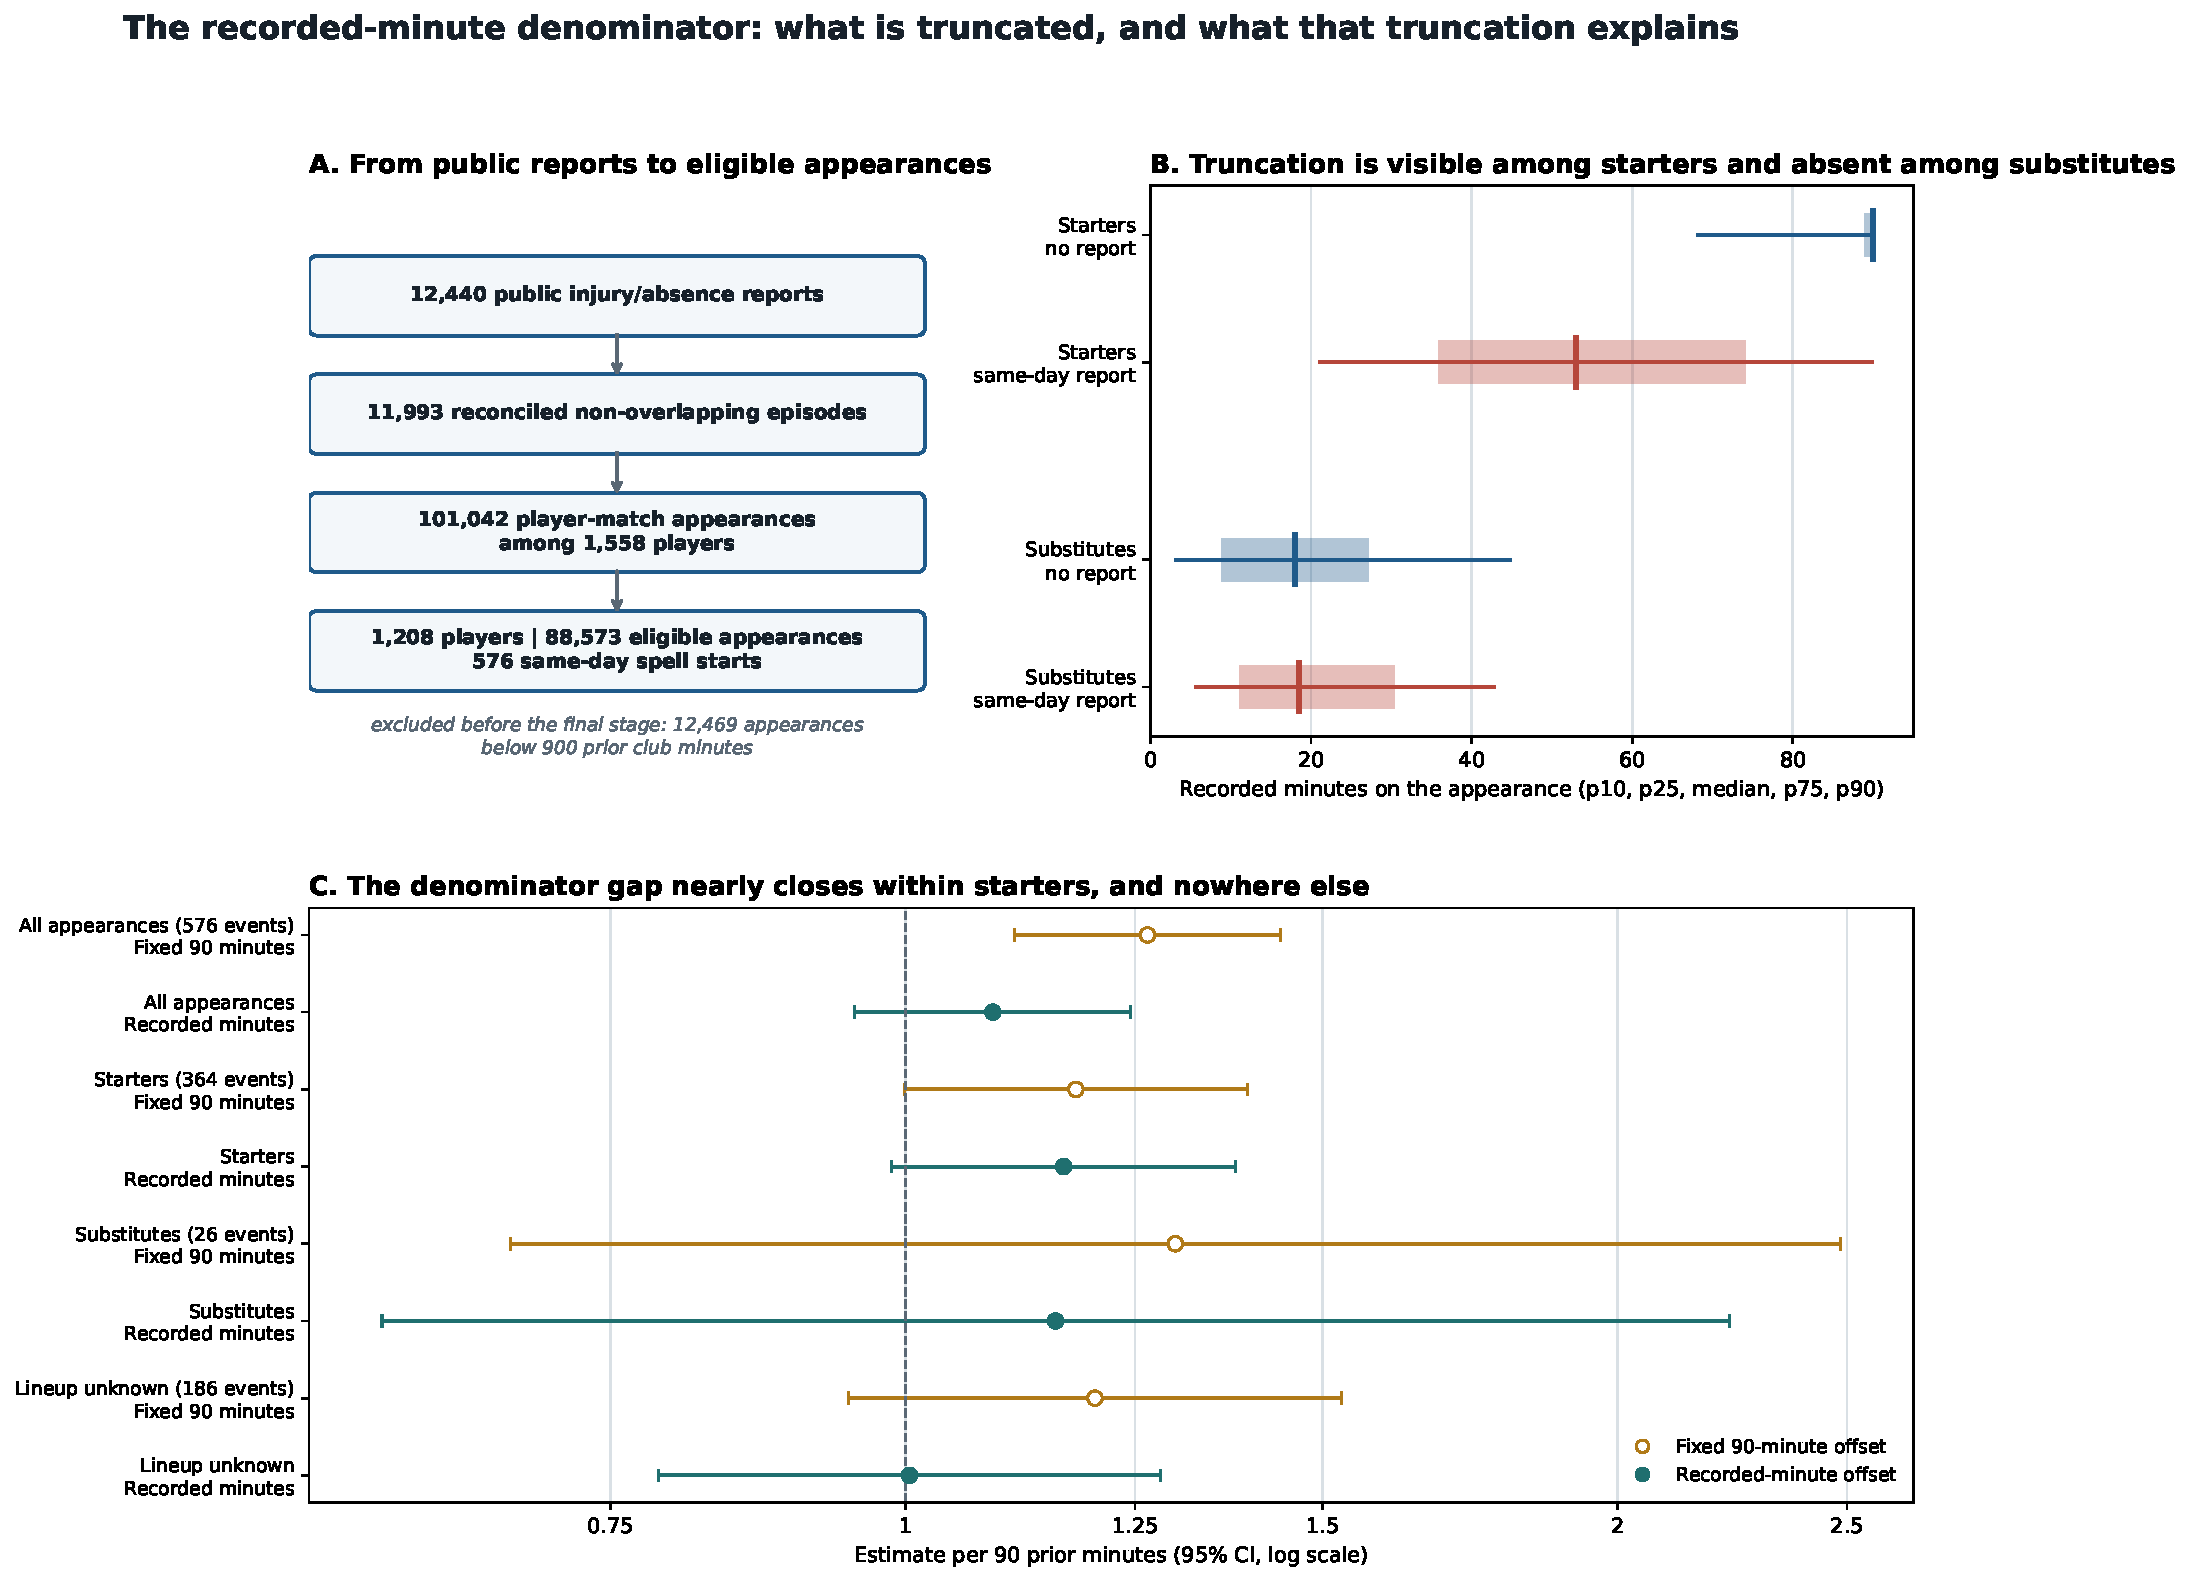
\includegraphics[width=\textwidth]{figures/J1_jsams_cohort_measurement.pdf}
\refstepcounter{figure}\label{fig:defects}
\end{figure}

\clearpage

\begin{figure}[htbp]
\centering
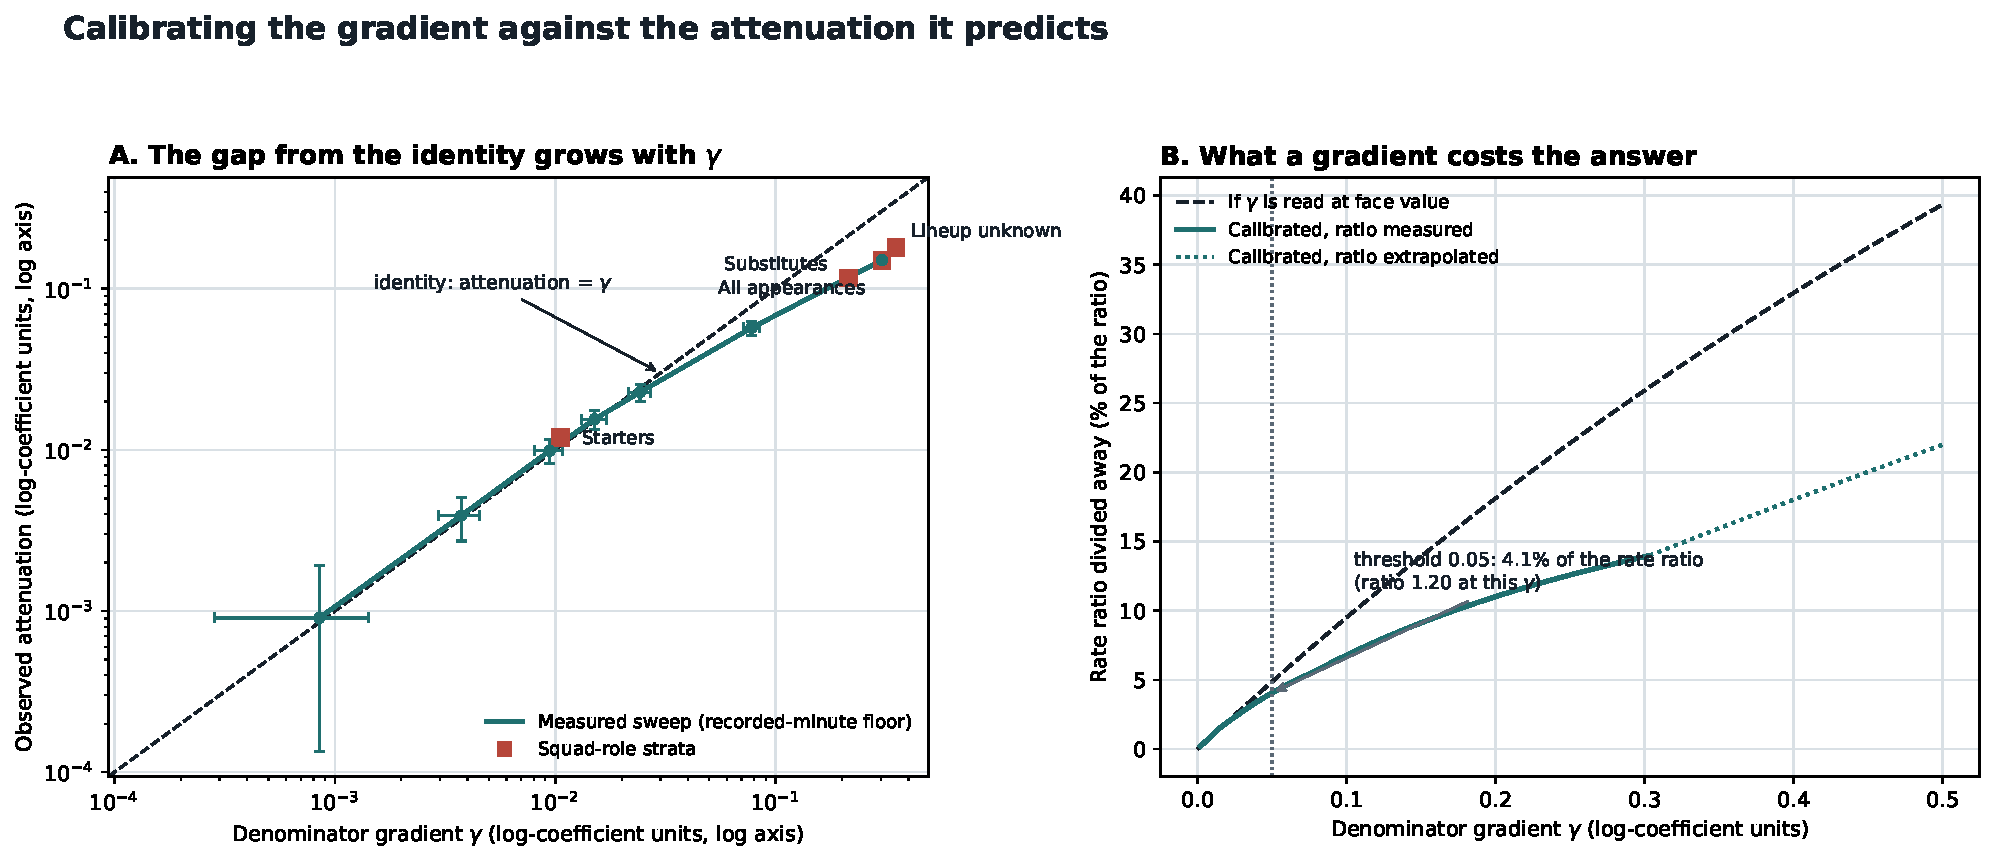
\includegraphics[width=\textwidth]{figures/J8_jsams_identity_calibration.pdf}
\refstepcounter{figure}\label{fig:calibration}
\end{figure}

\clearpage

\begin{figure}[htbp]
\centering
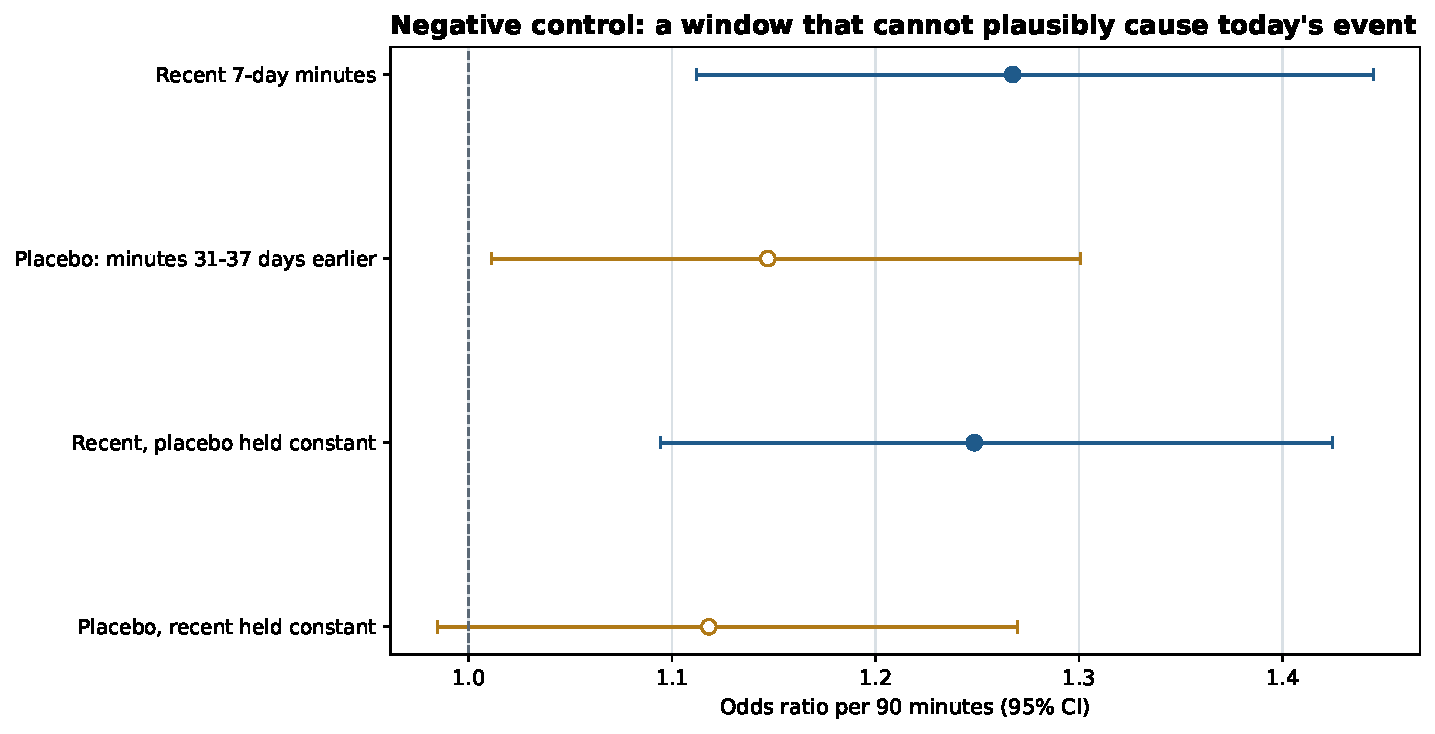
\includegraphics[width=0.86\textwidth]{figures/J5_jsams_negative_control_exposure.pdf}
\refstepcounter{figure}\label{fig:negative_control}
\end{figure}

\clearpage

\begin{figure}[htbp]
\centering
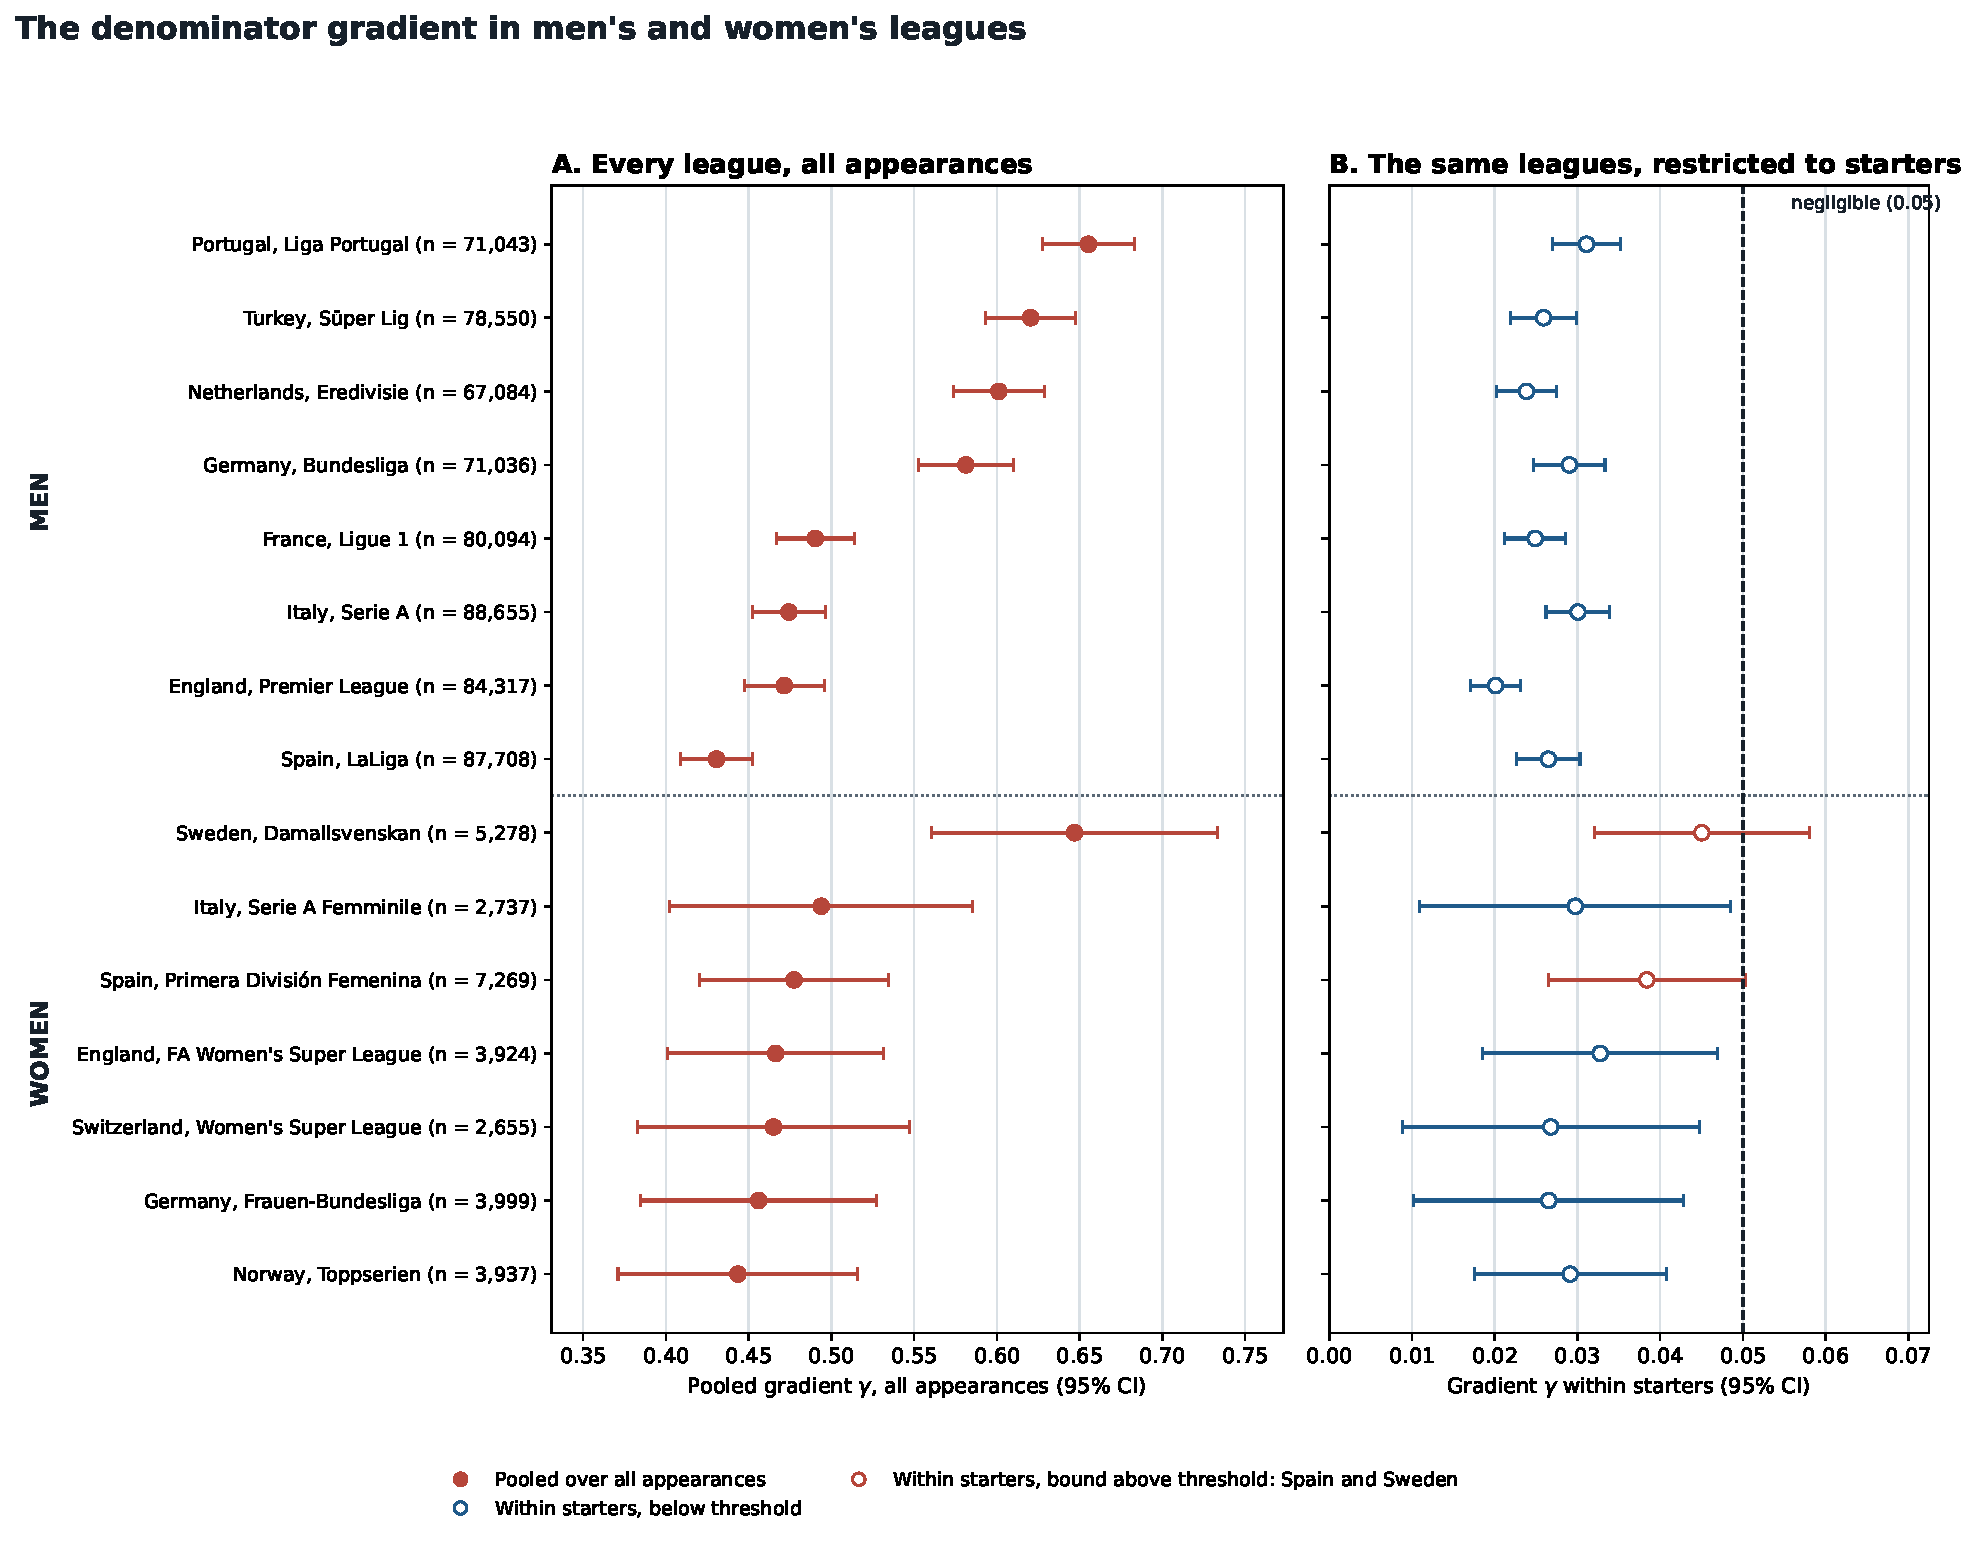
\includegraphics[width=\textwidth]{figures/J7_jsams_gradient_by_population.pdf}
\refstepcounter{figure}\label{fig:population}
\end{figure}

\clearpage

\begin{figure}[htbp]
\centering
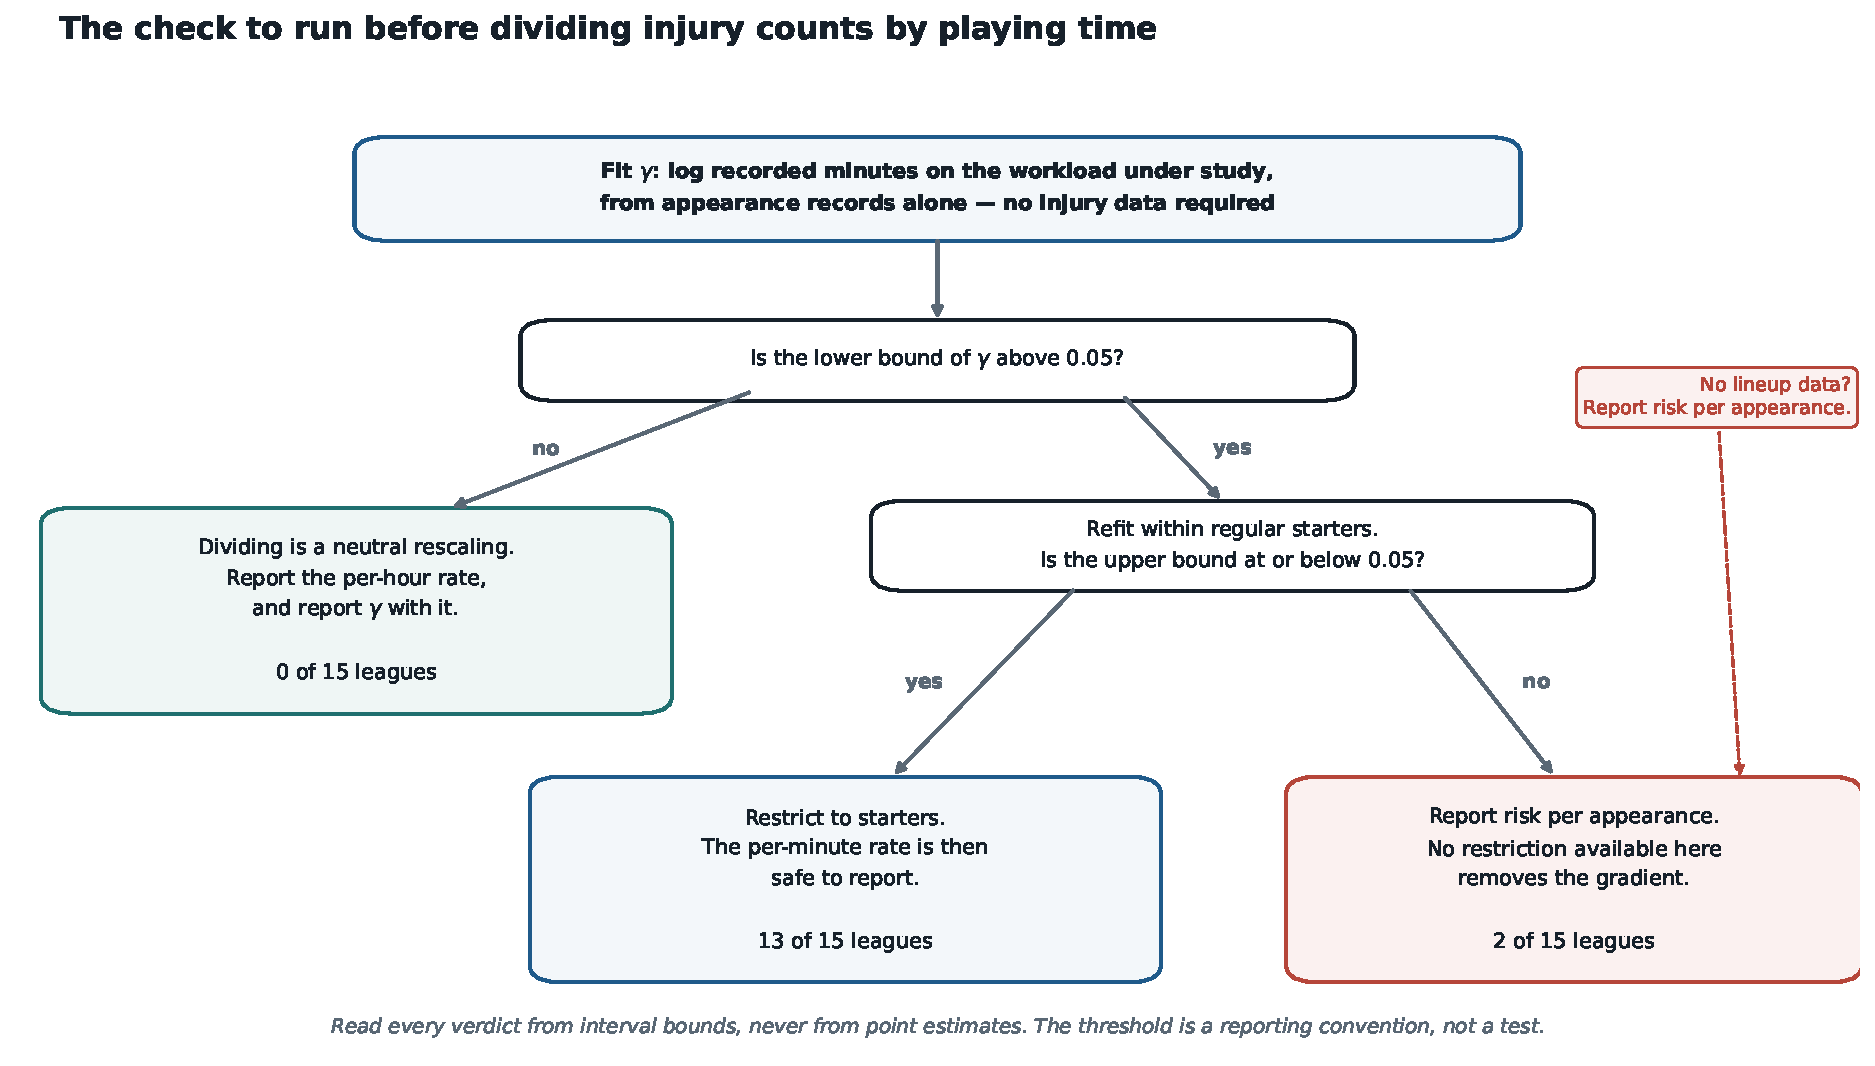
\includegraphics[width=\textwidth]{figures/J9_jsams_decision_rule.pdf}
\refstepcounter{figure}\label{fig:rule}
\end{figure}

\clearpage
\section*{Figure captions}

\noindent\textbf{Figure 1.} The two defects in the recorded-minute denominator, reference cohort. Panel A separates the 12,469 run-in exclusions from the retained cohort. Panel B gives the distribution of recorded minutes (p10, p25, median, p75, p90) by lineup role and event status: among starters the distribution shifts markedly when a same-day report is present, while among substitutes it does not, which is the signature of early withdrawal rather than a uniform shift. Starters without a report have an interquartile range of 89--90 minutes, so their box collapses to a line at this scale. Panel C refits the denominator comparison within squad role; fixed-90 and recorded-minute models are both Poisson with a log link on identical rows, so only the offset differs between them and both estimates are rate ratios. Panel C uses its own two colours, because it contrasts denominators rather than the event states contrasted in panel B. The pooled gap between those two models nearly closes within starters. These are associations between reported spell starts and recorded appearance length; they do not identify event time.

\vspace{0.6em}

\noindent\textbf{Figure 2.} Calibrating the gradient against the attenuation it predicts. Both panels are in log-coefficient units on the horizontal axis. Panel A plots the attenuation observed against the gradient $\gamma$, which the first-order identity of Section~2.3 predicts it will equal; the dashed line is that prediction. Both of its axes are logarithmic, so the identity remains the diagonal, a point's vertical distance below it is the log of the over-prediction ratio, and the intervals at the smallest floors are visible instead of vanishing into a corner. The teal line is a measured sweep: raising a floor on recorded minutes shrinks the variation the offset can act on, so $\gamma$ falls while the outcome, the exposure and the specification stay fixed. The ratio of predicted to observed attenuation is therefore measured rather than assumed constant, and it runs from 0.94 at $\gamma=0.001$ to 2.01 at $\gamma=0.303$. Squares mark the four squad-role strata for comparison. The expansion weights every appearance equally while the Poisson score weights by fitted means, which is why the two agree while $\gamma$ is small and diverge as it grows. Panel B converts a gradient into the share of the reported rate ratio a recorded-minute denominator removes, read naively off $\gamma$ and after calibration at that $\gamma$; the calibrated curve is solid where the ratio was measured and dotted beyond the swept range. Error bars on the sweep are the gradient's player-clustered interval (horizontal) and the attenuation's 1000-player-resample interval (vertical), and they widen as the floor rises because the surviving strata carry fewer events. At the negligible threshold of 0.05 the measured ratio is 1.20 (1.15 to 1.28) and the cost is 4.1\% (3.8 to 4.3) of the rate ratio. The curve is measured in this cohort: the ratio depends on the joint distribution of minutes, exposure and events, of which $\gamma$ is one summary, so an analyst fitting an outcome model should sweep their own data --- the sweep reuses the models already being fitted --- rather than borrow this curve.

\vspace{0.6em}

\noindent\textbf{Figure 3.} Negative-control exposure. Minutes played 31 to 37 days before an appearance share the player's reporting profile, club and durability, but their contribution to an injury reported today should be far smaller than the recent window's. Fitted alone the placebo window carries an association; with both windows in one model the recent window survives adjustment and the placebo window does not. The mutually adjusted comparison is the informative one, because a placebo association as large as the recent-window association would indicate persistent player-level reporting propensity rather than recent load. These are per-appearance logistic fits and therefore odds ratios, not the rate ratios of Figure 1C. That is deliberate and follows from this paper's own finding: a control for reporting propensity must not be passed through a denominator that carries the exposure gradient. Estimates are per 90 previous minutes with player-clustered 95\% intervals.

\vspace{0.6em}

\noindent\textbf{Figure 4.} The denominator gradient $\gamma$ in eight men's and seven women's European leagues, fitted from appearance records alone with no injury data of any kind. Panel A gives the pooled gradient over all appearances; panel B gives the gradient within starters on its own scale, because the two series differ by an order of magnitude and a shared axis renders the restricted intervals unreadable. Leagues are ordered by pooled gradient within population, and panel labels carry the number of appearances behind each estimate. Bars are 95\% confidence intervals from a covariance clustered on player identifier, and the dashed line in panel B marks the negligible threshold of 0.05, a reporting convention rather than a test. Men's leagues cover 628,487 appearances between 1 July 2017 and 7 April 2025 from a Transfermarkt-derived snapshot; women's leagues cover 29,799 appearances between 9 August 2024 and 16 November 2025, one complete season each, reconstructed from Soccerdonna match reports. The pooled gradient exceeds the threshold in all 15 leagues. The within-starter gradient falls below it in all eight men's leagues and in five of seven women's; in Spain and Sweden the within-starter interval reaches 0.050 and 0.058, drawn in the warning colour, so the decision rule returns risk per appearance for those two.

\vspace{0.6em}

\noindent\textbf{Figure 5.} The check to run before dividing injury counts by playing time, and where the fifteen leagues measured here land in it. The gradient is fitted from an appearance table alone --- player identifier, date, recorded minutes --- and needs no injury data, so the check can be run before any outcome model is specified. Every verdict is read from an interval bound rather than a point estimate. The second decision needs lineup data, which many public sources do not publish and which is missing for a quarter of our own reference cohort; the side note gives those readers their route, which is to report risk per appearance. The threshold of 0.05 is a reporting convention, not a test, and corresponds to about 4\% of the rate ratio at that gradient (Figure~\ref{fig:calibration}); a reader preferring a different tolerance can substitute one, which is why we report $\gamma$ with its interval whatever the verdict.

\end{document}
